%!TEX root=paper/thesis.tex
\chapter{Introduction}

\section{NIPS12 Introduction} \label{sec:nips12_introduction}

In real-world applications of visual object recognition, performance is time-sensitive.
In robotics, a small finite amount of processing power per unit time is all that is available for robust object detection, if the robot is to usefully interact with humans.
In large-scale detection systems, such as image search, results need to be obtained quickly per image as the number of items to process is constantly growing.
In such cases, an acceptable answer at a reasonable time may be more valuable than the best answer given too late.

\begin{figure}[ht!]
\center{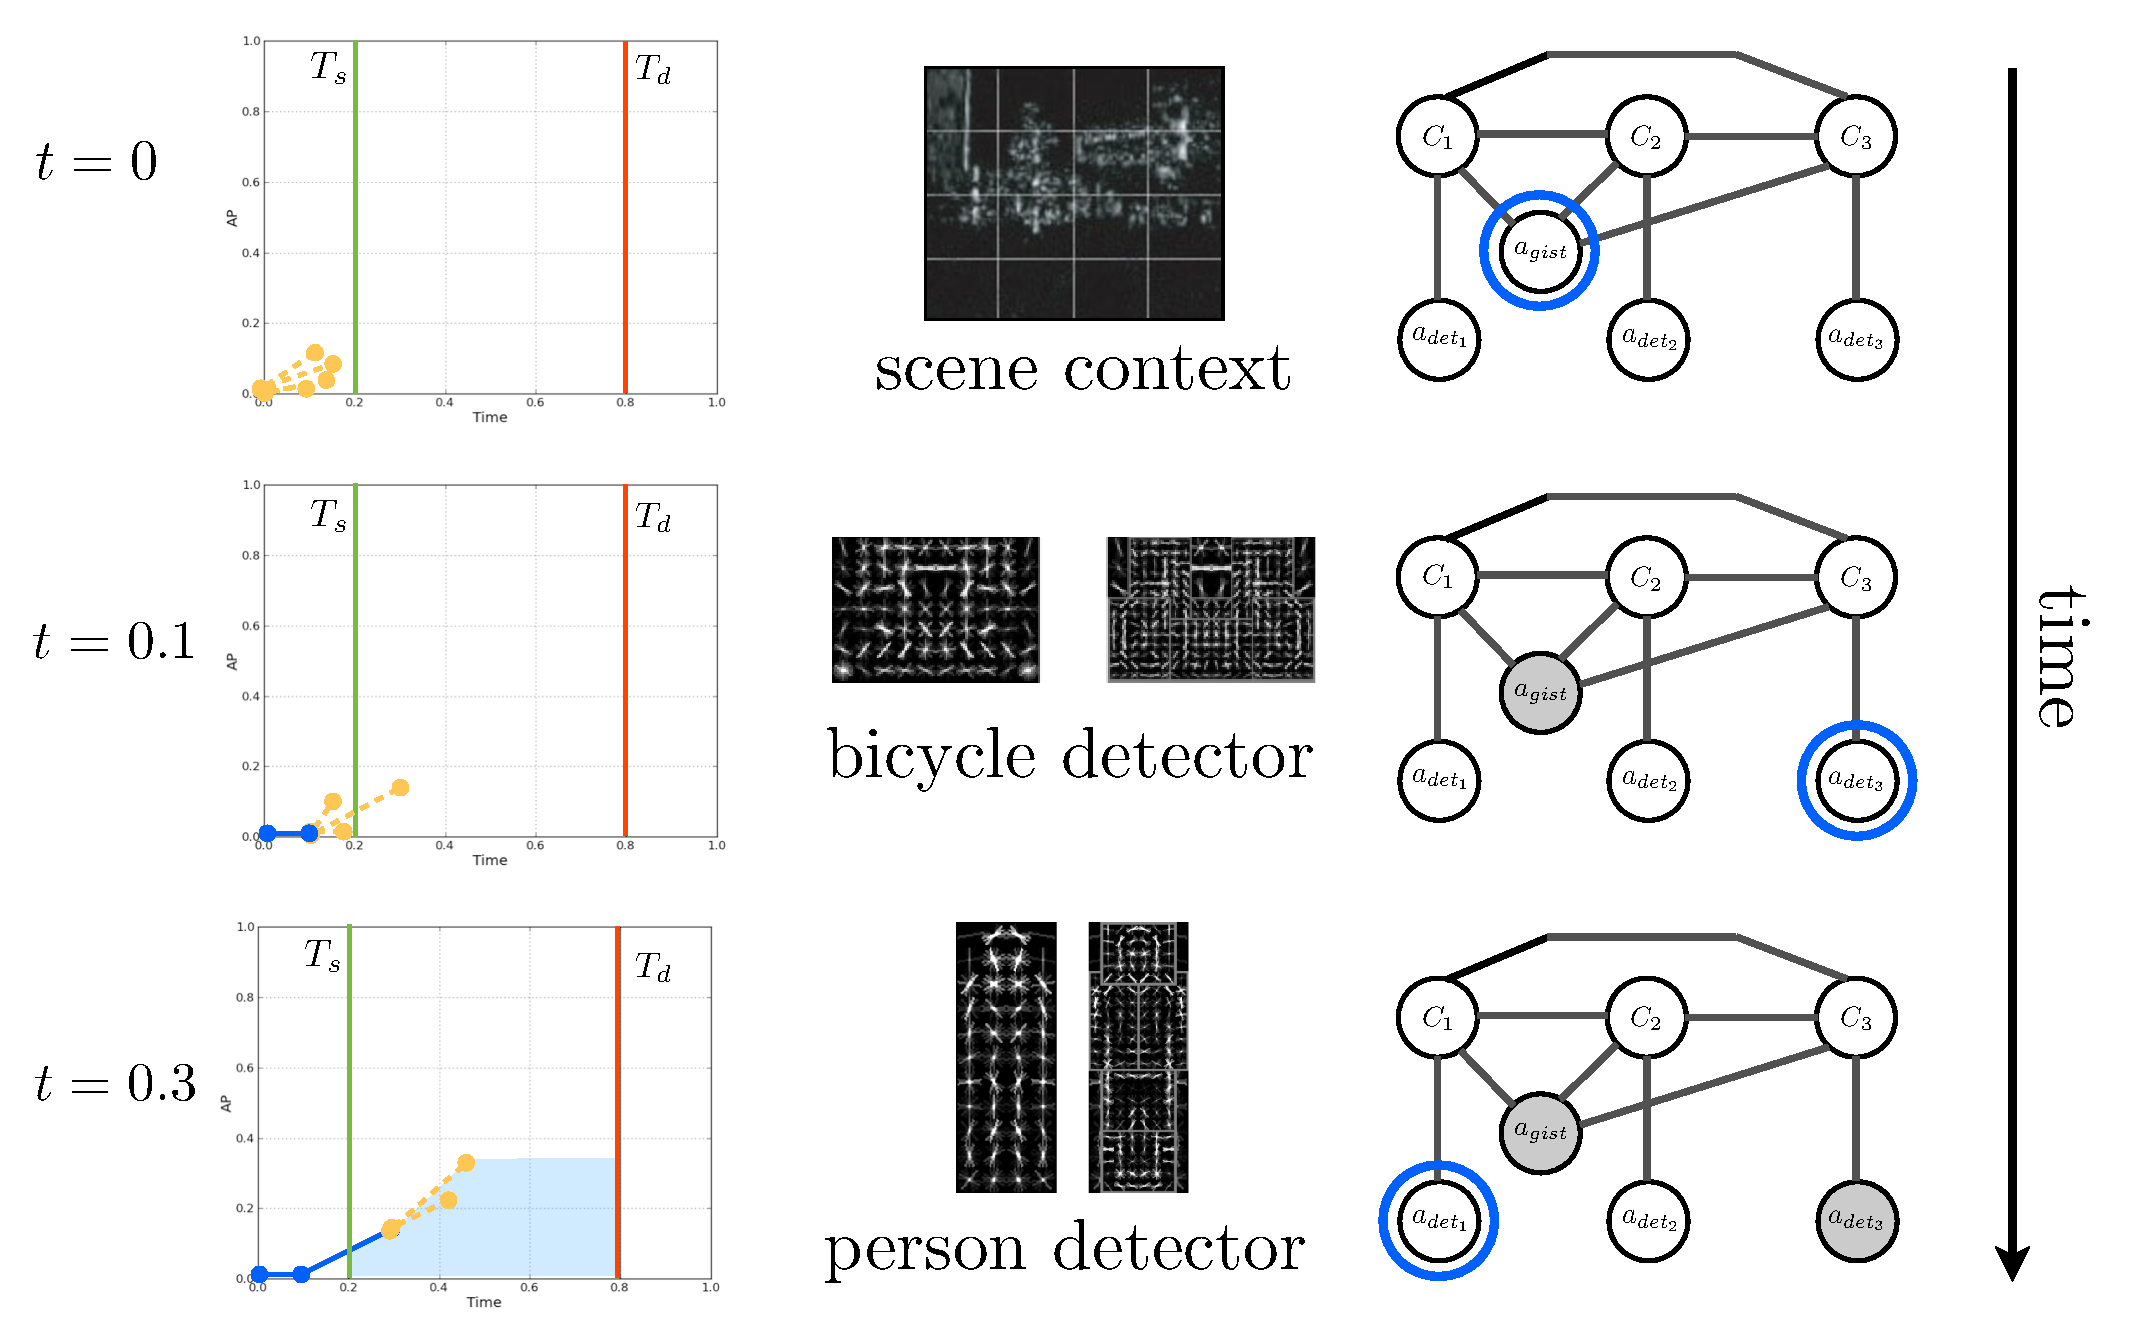
\includegraphics[width=0.86\linewidth]
    {../../../2011-2012/figures/figure1.pdf}}
  \caption{
A sample trace of our method.
At each time step beginning at $t=0$, potential actions are considered according to their predicted \emph{value}, and the maximizing action is picked.
The selected action is performed and returns \emph{observations}.
Different actions return different observations: a detector returns a list of detections, while a scene context action simply returns its computed feature.
The \emph{belief model} of our system is updated with the observations, which influences the selection of the next action.
The final evaluation of a detection episode is the area of the \emph{AP vs. Time} curve between given start and end times.
The value of an action is the expected result of final evaluation if the action is taken and the policy continues to be followed, which allows actions without an immediate benefit to be scheduled.
}
  \label{fig:figure1}
\end{figure}

A hypothetical system for vision-based advertising presents a case study: companies pay money to have their products detected in images on the internet.
The system has different values (in terms of cost per click) and accuracies for different classes of objects, and the queue of unprocessed images varies in size.
The detection strategy to maximize profit in such an environment has to exploit every inter-object context signal available to it, because there is not enough time to run detection for all classes.

What matters in the real world is timeliness, and either not all images can be processed or not all classes can be evaluated in a detection task.
Yet the conventional approach to evaluating visual recognition does not consider efficiency, and evaluates performance independently across classes.
We argue that the key to tackling problems of dynamic recognition resource allocation is to start asking a new question:
\emph{What is the best performance we can get on a budget?}

Taking the task of object detection, we propose a new \emph{timeliness} measure of performance vs. time (shown in Figure~\ref{fig:figure1}).
We present a method that treats different detectors and classifiers as black boxes, and uses reinforcement learning to learn a dynamic policy for selecting actions to achieve the highest performance under this evaluation.

Specifically, we run scene context and object class detectors over the whole image sequentially, using the results of detection obtained so far to select the next actions.
Evaluating on the PASCAL VOC dataset and evaluation regime, we are able to obtain better performance than all baselines when there is less time available than is needed to exhaustively run all detectors.

\section{NIPS12 Related Work}

\paragraph{Object detection}
The best recent performance has come from detectors that use gradient-based features to represent objects as either a collection of local patches or as object-sized windows \cite{Dalal2005,Lowe2004}.
Classifiers are then used to distinguish between featurizations of a given class and all other possible contents of an image window.
Window proposal is most often done exhaustively over the image space, as a ``sliding window''.

For state-of-the-art performance, the object-sized window models are augmented with parts \cite{Felzenszwalb2010a}, and the bag-of-visual-words models employ non-linear classifiers \cite{Vedaldi2009}.
We employ the widely used Deformable Part Model detector \cite{Felzenszwalb2010a} in our evaluation.
Some approaches use ``jump windows'' (hypotheses voted on by local features) \cite{Vedaldi2009,Vijayanarasimhan2011}, or a bounded search over the space of all possible windows \cite{Lampert2008a}.

None of the best-performing systems treat window proposal and evaluation as a closed-loop system, with feedback from evaluation to proposal.
Some work has been done on this topic, mostly inspired by ideas from biological vision and attention research~\cite{Butko2009,Vogel2008}.

Most detection methods train individual models for each class.
Work on inherently multi-class detection focuses largely on making detection time sublinear in the number of classes through sharing features \cite{Torralba2007,Fan2005}.

A post-processing extension to detection systems uses structured prediction to incorporate multi-class context as a principled replacement for non-maximum suppression \cite{Desai2009}.

\paragraph{Using context}
The most common source of context for detection is the \emph{scene} or other non-detector cues; the most common scene-level feature is the GIST \cite{Oliva-IJCV-2001} of the image.
We use this source of scene context in our evaluation.

Inter-object context has also been shown to improve detection \cite{Torralba2004}.
In a standard evaluation setup, inter-object context plays a role only in post-filtering, once all detectors have been run.
In contrast, our work leverages inter-object context in the action-planning loop.

A critical summary of the main approaches to using context for object and scene recognition is given in \cite{Galleguillos2010}.
For the commonly used PASCAL VOC dataset \cite{pascal-voc-2010}, GIST and other sources of context are quantitatively explored in~\cite{Divvala2009}.

\paragraph{Efficiency through cascades}
An early success in efficient object detection of a single class uses simple, fast features to build up a \emph{cascade} of classifiers, which then considers image regions in a sliding window regime \cite{Viola2004}.
Most recently, cyclic optimization has been applied to optimize cascades with respect to feature computation cost as well as classifier performance \cite{Chen-AISTATS-2012}.

Cascades are not dynamic policies: they cannot change the order of execution based on observations obtained during execution, which is our goal.

\paragraph{Anytime and active classification}
This surprisingly little-explored line of work in vision is closest to our approach.
A recent application to the problem of visual detection picks features with maximum value of information in a Hough-voting framework \cite{Vijayanarasimhan2010}.
There has also been work on active classification \cite{Gao-NIPS-2011} and active sensing \cite{Yu2009}, in which intermediate results are considered in order to decide on the next classification step.
Most commonly, the scheduling in these approaches is greedy with respect to some manual quantity such as expected information gain.
In contrast, we learn policies that take actions without any immediate reward.

\section{CVPR14 Introduction}

Anytime recognition is a core competence in human perception, mediating between reflexive recognition and deep analysis of visual input.
Human studies have produced evidence for coarse-to-fine processing of visual input as more time becomes available \parencite{Vanrullen-1996,Fei-Fei-Vision-2007,Mace-PloS-2009}.
The underlying mechanisms are unknown, with only a few attempts to explain the temporal dynamics (e.g. via sequential decision processes in \textcite{Hegde-Neuro-2008}).

While multi-class recognition in computer vision has achieved levels of performance that allow useful real-world implementation, state-of-the-art methods tend to be computationally expensive and insensitive to Anytime demands.
As these methods are applied at scale, managing their resource consumption (power or cpu-time) cost becomes increasingly important.
For tasks such as personal robotics, the ability to deploy varying levels of processing to different stimuli, depending on computational demands on the robot, also seems crucial.

For most state-of-the-art classification methods, different features are extracted from an image instance at different costs, and contribute differently to decreasing classification error.
Although ``the more features, the better'', high accuracy can be achieved with only a small subset of features for some instances---and different instances benefit from different subsets of features.
For example, simple binary features are sufficient to quickly detect faces \parencite{Viola2004} but not more varied visual objects, while the features most useful for separating landscapes from indoor scenes \parencite{Xiao-CVPR-2010} are different from those most useful for recognizing fine distinctions between bird species \parencite{Farrell-ICCV-2011}.

Computing all features for all images is infeasible in a deployment sensitive to Anytime needs, as each feature brings a significant computational burden.
To deal with this problem, we can set an explicit cost \emph{budget}, specified in terms of wall time or total power expended or another metric.
Additionally, we strive for \emph{Anytime} performance---the ability to terminate the classifier even before the cost budget is depleted and still obtain the best answer.
In this paper, we address the problem of selecting and combining a subset of features under an \emph{Anytime} cost budget.

To exploit the fact that different instances benefit from different subsets of features, our approach to feature selection is a sequential policy.
To learn the policy parameters, we formulate the problem as a Markov Decision Process (MDP) and use reinforcement learning methods.
With different settings of parameters, we can learn policies ranging from \textbf{Static, Myopic}---greedy selection not relying on any observed feature values, to \textbf{Dynamic, Non-myopic}---relying on observed values and considering future actions.

Since test-time efficiency is our motivation, our methods should carry little computational burden.
For this reason, our models are based on linear evaluations, not nearest-neighbor or graphical model methods.
Because different features can be selected for different instances, and because our system may be called upon to give an answer at any point during its execution, the feature combination method needs to be robust to a large number of different observed-feature subsets.
To this end, we present a novel method for learning several classifiers for different clusters of observed-feature subsets.

We evaluate our method on multi-class recognition tasks.
We first demonstrate on synthetic data that our algorithm learns to pick features most useful for the specific test instance.
We demonstrate the advantage of non-myopic over greedy, and of dynamic over static on this and the Scene-15 visual classification dataset.
Then we show results on a subset of the hierarchical ImageNet dataset, where we additionally learn to provide the most specific answers for any desired cost budget and accuracy level.

\section{CVPR14 Related Work}
\paragraph{Feature combination and selection.}
\emph{Boosting} is a method for combining weak learners into a more powerful classifier \parencite{Hastie2009}.
A popular use of boosting is in introducing non-linearities by training depth-limited decision trees as weak learners---the boosting trick.
For SVM-based classifiers, \emph{Multiple Kernel Learning} (MKL) provides a way to train classifiers using an automatically weighted combination of kernels \parencite{Lanckriet2004}.
It has been shown that MKL is outperformed by boosting single-kernel classifiers \parencite{Gehler2009}.
Of course, if all classifiers are linear, then combining outputs of classifiers trained on different feature channel with another classifier is equivalent to training one classifier on all features at once.
\todo{What about learning a \emph{non-linear} second classifier on top of the weak learner scores---any papers?}

\paragraph{Static test-time efficient feature selection.}
The simplest way to limit the number of features used at test time is to $L_1$-regularize.
This method does not explicitly consider feature cost, nor is it able to evaluate features one by one, or to give an answer before all features are computed.

A well-known method to evaluate features sequentially is the cascaded boosted classifier of Viola \& Jones \parencite{Viola2004} (updated by Bourdev \& Brandt \parencite{Bourdev-CVPR-2005} with a soft threshold), which is able to quit evaluating an instance before all features are computed---but feature cost was not considered.
The cost-sensitive cascade of Chen et al.\ \parencite{Chen-AISTATS-2012} optimizes stage order and thresholds to jointly minimize classification error and feature computation cost.
Xu et al.\ \parencite{Xu-ICML-2012} and Grubb \& Bagnell \parencite{Grubb-AISTATS-2012} separately develop a variant of gradient boosting for training cost-sensitive classifiers; the latter prove near-optimality of their greedy algorithm with submodularity results.
Their methods are tightly coupled to the stage-wise regression algorithm.

\paragraph{Dynamic test-time efficient feature selection.}
The above methods learn an efficient but \emph{fixed} order for evaluating features given a test instance.

Gao \& Koller \parencite{Gao-NIPS-2011} propose a method for \emph{active classification}: myopically selecting the next feature based on expected information gain given the values of the already selected features.
The method is based on locally weighted regression, highly costly at test time.
Ji \& Carin \parencite{Ji-PR-2007} also formulate cost-sensitive feature selection generatively, as an HMM conditioned on actions, but select actions myopically, again at signficant test time cost.

Karayev at al.\ \parencite{Karayev-NIPS-2012} propose a reinforcement learning approach for selecting object detectors; they rely on expensive test-time inference in a graphical model to combine observations.
Dulac-Arnold et al.\ \parencite{DulacArnold-ML-2012} present another MDP-based solution to ``datum-wise classification'', with an action space comprised of all features and labels, recently extended to region-based processing \parencite{DulacArnold-ICLR-2014}.
He He et al.\ \parencite{HeHe-ICMLW-2012} also formulate an MDP with features and a single classification step as actions, but solve it via imitation learning of a greedy policy.
Benbouzid et al.\ \parencite{Benbouzid-ICML-2012} formulate an MDP that simply extends the traditional sequential boosted classifier with an additional \emph{skip} action, significantly limiting the space of learnable policies (\parencite{Trapeznikov-ML-2012} provides another variation on this problem).
Although \parencite{Karayev-NIPS-2012} targets \emph{Anytime} performance, their inference procedure is prohibitively expensive for test-time use in a general classification task.
In contrast, our fast linear method allows direct specification of the Anytime cost budget.

\emph{Label trees} also guide an instance through a tree of classifiers; their structure is determined by the confusion matrix or learned jointly with weights \parencite{Deng-NIPS-2011}.
Xu et al.\ \parencite{Xu-ICML-2013} learn a cost-sensitive binary tree of weak learners using an approach similar to the cyclic optimization of \parencite{Chen-AISTATS-2012}.
Less directly related---but exciting for its novelty---is the work of \parencite{Weiss-ICCV-2013}, who apply simple introspection to structured models for a significant speedup of human pose estimation.
Another exciting direction is theoretical analysis of near-optimal policies with humans in the loop \parencite{Chen-2014-ICML}.
